\documentclass[../main.tex]{subfiles}
\begin{document}
\chapter{逻辑回归}
% Logistic Regression

\section{分类问题}
\paragraph{分类问题的分类}\begin{itemize}
    \item 二元分类问题,\(y∈{0, 1}\)
    \item 多元分类问题,\(y∈{0, 1, 2}\)
\end{itemize}

\section{假设表示}
% Hypothesis Representation
在线性回归中使用\(h_θ(x) = θ^Tx\)作为假设,在二分类的逻辑回归中使用\(h_θ(x) = g( θ^Tx) = \frac{1}{1+e^{-θ^Tx}}\)作为假设,其中\(g\)是逻辑函数\textbf{Logistic function}\(g(z) = \frac{1}{1+e^{-z}}\),一个S型函数。
\begin{figure}[H]
    \centering
    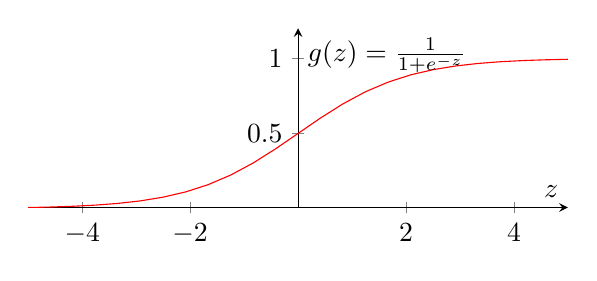
\begin{tikzpicture}
    \begin{axis}[
        axis y line = center,
        axis x line = middle,
        y post scale = 0.4,
        ytick = {0.5, 1},
        ymax = 1.2,
        xlabel=\(z\),
        ylabel={\(g(z) = \frac{1}{1+e^{-z}}\)}
    ]
    \addplot[color=red,]{1/(1+exp(-x))};
    \end{axis}
\end{tikzpicture}
\end{figure}

对于给定的输入,\(h_θ(x)\)表示\(y=1\)的可能性,而且有:\(P(y=0|x) = 1 - P(y=0|x) \)

\section{决策边界}
% Decision Boundary
预测值\(y' = \begin{cases}
    1 & h_θ(x)≥0.5, 即 θ^Tx ≥ 0   \\
    1 & h_θ(x)<0.5, 即 θ^Tx < 0 \\
\end{cases}\),
那么\(θ^Tx\)就是决策边界,在两个特征的二元分类中,它就是一条直线(关于特征)。同时,逻辑回归也可以选择多项式回归,比如一个近似圆的边界(关于原始特征),可以选择\(θ^Tx = θ_0 + θ_1x_1 + θ_2x_2 + θ_3x_1^2 + θ_4x_2^2\)。

\section{代价函数}
\(Cost(h_θ(x), y) = \frac{1}{2}(h_θ(x) - y)^2\)不适合\(h_θ(x)=\frac{1}{1+e^{-θ^Tx}}\),因为这时代价函数是一个非凸函数(non-convex),在梯度下降得过程中很容易陷入局部最优解。这时选择\(Cost(h_θ(x), y) = \begin{cases}
    -\log(h_θ(x))    & y = 1 \\
    -\log(1- h_θ(x)) & y = 0
\end{cases}\)

\begin{figure}[H]
    \centering
    \begin{tikzpicture}
    \begin{axis}[
        scale = 0.7,
        axis y line = center,
        axis x line = middle,
        legend pos = outer north east,
        xlabel=\(h_θ(x)\),
        ylabel={\(Cost\)},
    ]
    \addplot[color=blue, domain=0.01:1, samples=99]{-ln(x)};
    \addlegendentry{\(y = 1\)}
    \addplot[color=red, domain=0:0.99, samples=99]{-ln(1-x)};
    \addlegendentry{\(y = 0\)}
    \end{axis}
\end{tikzpicture}
\end{figure}

\section{简化代价函数和梯度下降}
因为y总是等于1或0,所以可以进一步简化代价函数:
\begin{align*}
    J(θ) & = \frac{1}{m}\sum\limits_{i=1}^{m}Cost(h_θ(x^{(i)}), y^{(i)})                                   \\
         & = \frac{1}{m}\sum\limits_{i=1}^{m}-y^{(i)}\log(h_θ(x^{(i)})) + (y^{(i)}-1)\log(1- h_θ(x^{(i)}))
\end{align*}


梯度下降算法一样的:\\
\begin{algorithm}[H]
    initialization\;
    \While{not convergence}{
        \(θ_j ← θ_j - α\frac{∂}{∂θ_j}J(θ)\) (j=0,1,\ldots, n)\;
    }
\end{algorithm}
重点在与求导代价函数:
% 没有求
\begin{align*}
    \frac{∂}{∂θ_j}J(θ) & = \frac{1}{m}\sum\limits_{i=1}^{m}(h_θ(x^{(i)}) - y^{(i)})x^{(i)_j}
\end{align*}
和线性回归代价函数的求导在形式上相同,注意的是假设函数是不同的

\subsection{代价函数推导}

使用最大似然法,写出似然函数:\begin{align*}
    L(θ) & = P(y|X; θ)                                                                  \\
         & = \prod\limits_{i=1}^{m}P(y^{(i)}|x^{(i)};θ)                                \\
         & = \prod\limits_{i=1}^{m}h_θ(x^{(i)})^{y^{(i)}} (1-h_θ(x^{(i)})^{1- y^{(i)}})
\end{align*}
同时对两边取对数:
\begin{align*}
    \log L(θ) & = \frac{1}{m}\sum\limits_{i=1}^{m}-y^{(i)}\log(h_θ(x^{(i)})) + (y^{(i)}-1)\log(1- h_θ(x^{(i)}))
\end{align*}

\section{高级优化}
% Advanced Optimization
梳理梯度下降:
\begin{enumerate}
    \item minimize cost
    \item 计算偏导数\(\frac{∂}{∂θ_j}J(θ)\),如果要监控\(J(θ)\)的收敛情况,还需要计算\(J(θ)\)
    \item 修正θ
\end{enumerate}
优化的思路在于更高效的计算\(\frac{∂}{∂θ_j}J(θ)\)、\(J(θ)\),更有效的调整学习率。更优秀(最优化)也更复杂的三种算法:
\begin{itemize}
    \item \textbf{共轭梯度法}
    \item \textbf{变尺度法 BFGS}
    \item \textbf{限制变尺度法 L-BFGS}
\end{itemize}
这三种算法有许多优点:
\begin{itemize}
    \item 自动选择一个好的\(α\)。它们使用\textbf{线性搜索 line search}算法,自动尝试不同的学习速率。
    \item 更快的收敛。
\end{itemize}
老师的建议:如果不是特定领域的专家,不必细致的研究这个领域的问题,明晰概念、特点,直接调用别人高效的实现就好了,就像我们不必编写计算平方根、逆矩阵的代码。


而使用这三种算法很简单,只需要你给出\textbf{cost function}和\textbf{gradient function}。

\section{多类别分类:一对多}
% Multiclass Classification One-vs-all
对于一对多的多类别分类,若类有\(r\)个,则可以将其转化为\(r\)个二元分类,对于二元分类,\(h\)表示结果为1(positive)的概率,那么在多个二元分类中选择概率最大的那个作为结果即可。


\end{document}